\documentclass[11pt]{article}

\usepackage[margin=1in]{geometry}
\usepackage{listings}
\usepackage{graphicx}
\usepackage{subfigure}
\usepackage{subcaption} % For subfigures
\usepackage{float} % for H option in figures
\usepackage{url}
\usepackage{float}
\usepackage{amsfonts}
\usepackage{hyperref}
\usepackage{amsmath}

\usepackage{biblatex} %Imports biblatex package
\addbibresource{../../../source/bibliography.bib} %Import the bibliography file

\setlength{\parindent}{0pt}

\title{What is a U-Net?}
\author{Anton Zhitomirsky}

\begin{document}

\maketitle

This is a sumamry of the contents of the file \cite{U-Net} and example of its implementation (from scratch and from the github)

\section{The architectural background} 

\begin{figure}[H]
    \centering
    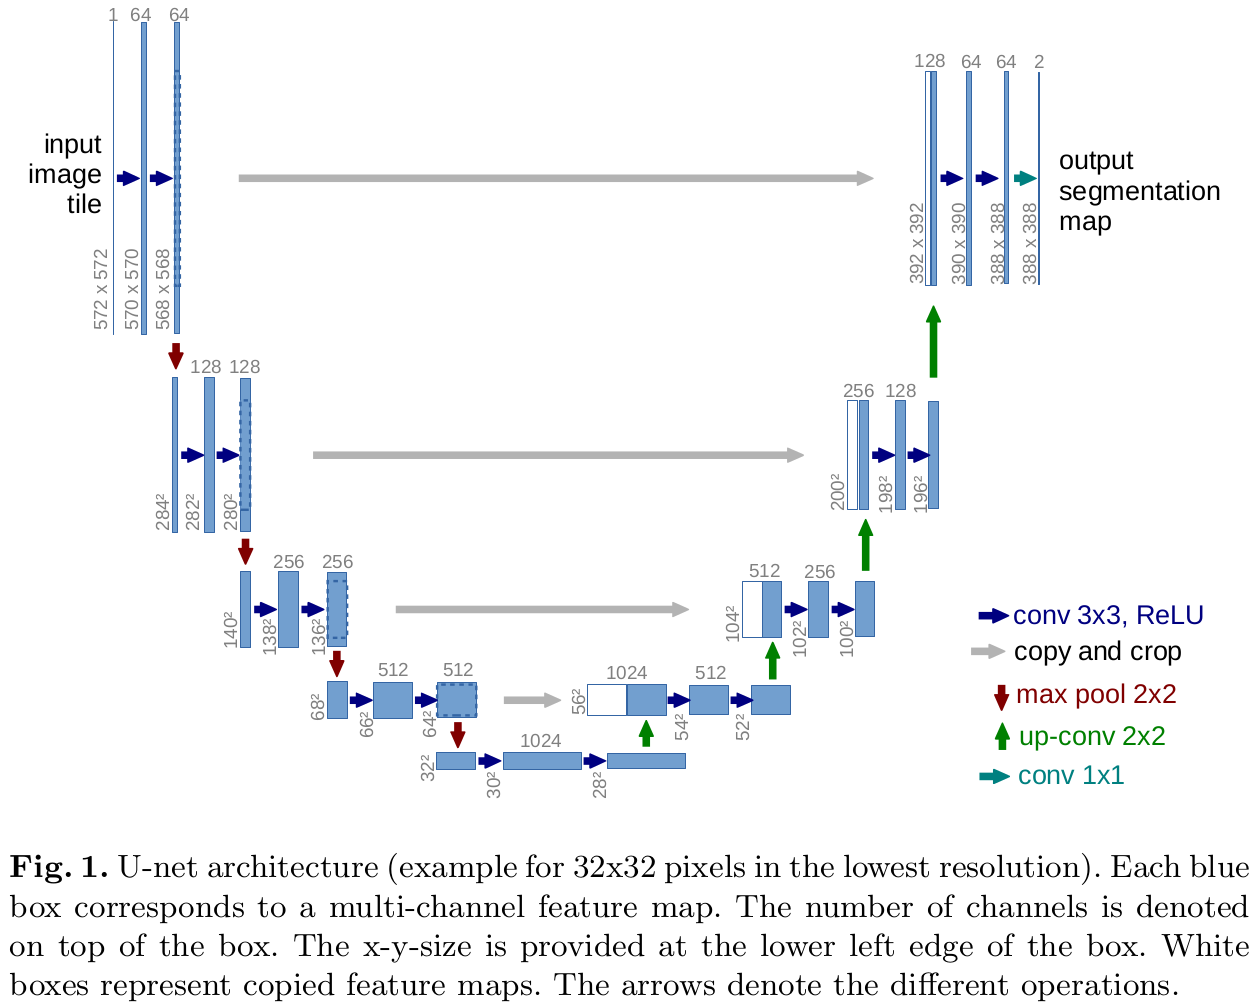
\includegraphics[width=\linewidth]{images/u-net.png}
    \caption{U-Net architecture taken from \cite{U-Net}}
    \label{fig:u-net-architecture}
\end{figure}

The U-Net is an adaption of another network \cite{fully-CNNs-for-semantic-segmentation}. We first discuss the architecture of the approach which is shown in Figure \ref{fig:u-net-architecture}.

\subsection{Method}

Most of the method can be seen by referencing the Legend of Figure \ref{fig:u-net-architecture}. It's worth noting that when we expand our features out we concatenate it with the correspondingly cropped feature map from the contracting path, and two 3x3 convolutions. The cropping is required due to the loss of border pixels in every convolution. At the final layer a 1x1 convolution is used to map each 64-component feature vector to the desired number of classes.

It is advised that you choose dimensions of an image that are even so that there is seamless tiling of the output segmentation map.

\subsection{Training}

This network favours large input tiles over a large batch size and hence they have reduced the batch to a single image. Accordingly they use a high momentum (0.99) such that a large number of the previously seen training samples determine the update in the current optimization step.

\subsubsection{Energy Function}

The energy function is computed by a pixel-wise soft-max (\ref{eq:soft-max}) over the final feature map combined with the cross entropy loss function (\ref{eq:cross-entropy}). 

\begin{equation}
    p_k(\textbf{x}) = \frac{\exp(a_k(\textbf{x}))}{\sum^K_{k'=1}\exp(a_{k'}(\textbf{x}))} \label{eq:soft-max}
\end{equation}

\begin{itemize}
    \item $a_k(\textbf{x})$ denotes the activation in feature channel $k$ at the pixel position $\textbf{x} \in \Omega, \Omega \subset \mathbb{Z}^2$
    \item $K$ is the number of classes
    \item $p_k(\textbf{x})$ is the approximated maximum-function ($\approx 1$ for the $k$ that has the maximum activation $a_k(\textbf{x})$ and $\approx 0$ for all other $k$)
\end{itemize}

\begin{equation}
    E = \sum_{\textbf{x} \in \Omega} w(\textbf{x})\log(p_{l(\textbf{x})}(\textbf{x})) \label{eq:cross-entropy}
\end{equation}

\begin{itemize}
    \item Cross Entropy penalizes at each position the deviation of $p_l(\textbf{x})(\textbf{x})$ from 1 using $E$
    \item $l : \Sigma \rightarrow \{1, \cdots, K \}$ is the true label of each pixel
    \item $w : \Sigma \rightarrow \mathbb R$ is a weight map which gives some pixels more importance in training. More details in paper.
\end{itemize}

\subsection{Conclusion}

The resulting architecture is symmetric in its expansive path as it is to its contracting path which yields its notorious u-shaped name. It doesn't contain any fully connected layers and only uses the valid part of each convolution (the segmentation map only contains the pixels, for which the full context is available in the input image).

\begin{figure}[H]
    \centering
    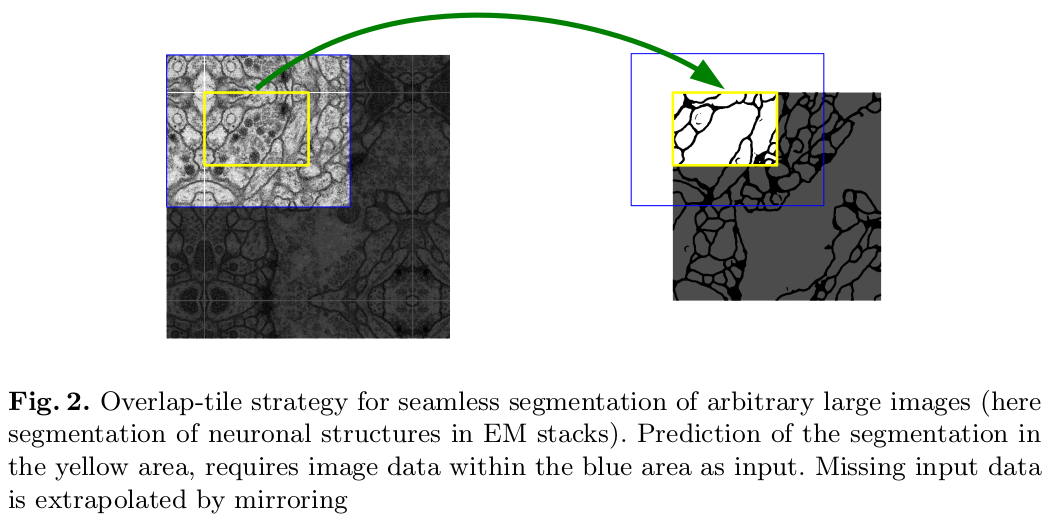
\includegraphics[width=\linewidth]{images/overlap-tile.png}
    \caption{Overlap figure taken from \cite{U-Net}}
    \label{fig:overlap-tile}
\end{figure}

It takes advantage of the overlap-tile strategy (Figure \ref{fig:overlap-tile}). This is result of passing through the features received at each level and passing it horizontally through to the upsampled level on the opposite side of the network.

\subsection{Considerations}

"Tasks where little training data is available, we use excessive data augmentation by applying elastic deformations to the available training images. This allows the network to learn invariance to such deformations, without the need to see those transformations in the annotated image corpus".

This might mean that for our purpose we may squash, stretch and transform the inputs to simulate different human phsiology yet maintain the same relative architecture.

\section{Implementation}

\section{Proposed extensions for the U-Net}

This section has been left as a TODO.

\subsection{Residual connections}

\subsubsection{\cite{identity-mappings-drns}}

This paper suggests that the forward and backward signals can be directly propagated from one block to any other block when using identity mappings as the skip conenctions and after-addition activation. code available at \href{https://github.com/KaimingHe/resnet-1k-layers/blob/master/resnet-pre-act.lua}{GitHub}.

\begin{figure}[H]
    \centering
    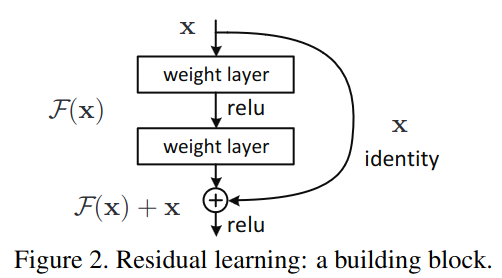
\includegraphics[width=0.4\linewidth]{images/residualArchitecture.png}
    \caption{Typic resudial network taken from \cite{drn-for-image-recognition}}
    \label{residual-architecture}
\end{figure}

The typical residual network as in Figure \ref{residual-architecture} makes training very deep networks easier than previous iterations. The formula typically follows 

\begin{align}
    \textbf{y}_l &= h(\textbf{x}_l) + F(\textbf{x}_l, W_l) \\
    \textbf{x}_{l+1} &= f(\textbf{y}_l)
\end{align}

$\textbf{x}_l$ and $\textbf{x}_{l+1}$ are input and output of the $l$-th unit, and F is a residual function. Above, 
$h(x_l)=x_l$ is an identity funciton. 

\subsubsection{\cite{v-net}}

\subsection{Dense connections}

\cite{tiramisu-densenet}

\subsection{Attention Mechanisms}

\cite{attention-u-net}

\printbibliography

\end{document}